%% Overleaf			
%% Software Manual and Technical Document Template	
%% 									
%% This provides an example of a software manual created in Overleaf.

\documentclass{ol-softwaremanual}

% Packages used in this example
\usepackage{graphicx}  % for including images
\usepackage{microtype}% for typographical enhancements
\usepackage{minted}    % for code listings
\usepackage{amsmath}   % for equations and mathematics
\setminted{style=friendly,fontsize=\small}
\renewcommand{\listoflistingscaption}{List of Code Listings}
\usepackage{hyperref}  % for hyperlinks
\usepackage[a4paper,top=4.2cm,bottom=4.2cm,left=3.5cm,right=3.5cm]{geometry} % for setting page size and margins
\usepackage{dirtree}
\usepackage{listings}
% Custom macros used in this example document
\newcommand{\doclink}[2]{\href{#1}{#2}\footnote{\url{#1}}}
\newcommand{\cs}[1]{\texttt{\textbackslash #1}}
\setlength{\parindent}{0em}
\setlength{\parskip}{0.8em}

% Frontmatter data; appears on title page
\title{Technical Manual \\Dynamic Positioning lab - TMR4243}
\version{2.0.0}
\author{Mathias Solheim}
\softwarelogo{
\includegraphics[width=8cm]{logo}}

\begin{document}

\maketitle

\tableofcontents
\listoflistings
\newpage

\section{Introduction}

This document provides aims to provide the necessary technical insight to utilize the software and hardware provided in the Dynamic Positioning lab of the course TMR4243 - Marine Control Systems II. The lab introduces the C/S (Cybership) Enterprise, which is a model scale tug boat fitted with a Raspberry Pi embedded computer and a ROS based control system. 


\subsection{Robot Operating Software}

This section will provide a brief introduction to the main concepts and advantages of the operating software used in the Marine Cybernetics lab; the \textit{Robot Operating System} (ROS).

Introduced in 2007, the Robot Operating System is an open source project that provides tools, libraries, and conventions for robot applications. It functions as a meta-operating system (OS)  handling services you would expect from a conventional OS. These include hardware abstraction, message-passing between processes and package management. 

A ROS process is represented as a node in a graph architecture. Nodes are connected to edges known as topics, through which they can pass messages to one another. They can also provide and make service calls of each-other and send or retrieve data from a common parameter server known as the ROS-master. The ROS-master registers all active nodes to itself, and establishes the peer-to-peer communication network of the nodes. Figure \ref{fig:ros-arch} illustrates the basic peer-to-peer communication of a ROS-system.


\begin{figure}[h]
    \centering
    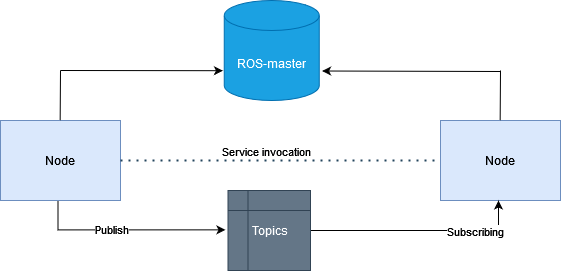
\includegraphics[width=0.8\textwidth]{ROS-diag.png}
    \caption{Basic ROS concept}
    \label{fig:ros-arch}
\end{figure}

This decentralized architecture is the main strength of ROS, as it allows nodes to be run on separate, networked hardware.

As each node-process is isolated and messages passed between standardized, the implementation language of the node is also irrelevant. Effectively this means that you can run one or more nodes written in C++ in conjunction with nodes written in, for example, Python. This ties in with the last strength; the ROS ecosystem. As an open source project ROS offers a plethora of easy and accessible software for robots, making the integration of sensors a simple task. Most hardware comes with ROS-support either from the manufacturer or a third party individual. As mentioned before, the software language is irrelevant, so one can easily download a C++ ROS-driver and run it with a mostly Python-based system. 

\section{Hardware}

As part of the lab you will be provided with the following hardware: 

\begin{enumerate}
    \item Raspberry Pi 4b computer
    \item A laptop running Ubuntu
    \item Dualshock 4 wireless controller
\end{enumerate}


\section{Software Prerequisites}
\begin{itemize}
    \item Python 3.8.3+
    \item Visual Studio Code, with the remote SSH-extension
    \item A PC with an Ethernet-port or an ethernet-adapter. 
\end{itemize}

The following are not required, but can be beneficial in work: 

\begin{itemize}
    \item A PC running Ubuntu
    \item PlotJuggler, a visualization tool
    \item bagpy, a tool for reading and plotting from ROS bag files.
\end{itemize}

The necessary equipment provided to you will come pre-installed with all the relevant software.

\section{Networking}

Connect the Raspberry Pi to your computer using an ethernet cable. Then, set the ethernet network settings on \textbf{your} computer to

\begin{itemize}
    \item IP: 192.168.1.1
    \item Subnet mask: 255.255.255.0
\end{itemize}

A quick how-to for Windows 10 is found \underline{\href{https://se.mathworks.com/help/supportpkg/usrpradio/ug/configure-ethernet-connection-manually-on-windows-10.html}{here}}. To verify the connection to raspberry pi, open up your preferred command-line tool and run the following command: 

\begin{lstlisting}[language=bash,basicstyle=\mlttfamily, breaklines=true]
  $ ping 192.168.1.2
\end{lstlisting}

where $192.168.1.2$ is the IP of the Raspberry Pi. If  the RPi responds you can SSH onto it and run files via the terminal. Simply run the command

\begin{lstlisting}[language=bash,basicstyle=\mlttfamily, breaklines=true]
  $ ssh pi@192.168.1.2
\end{lstlisting}

Most likely you will then be prompted for a password. All the RPi's have \textbf{\textit{marin33}} as the designated password.

\section{How to ROS: A step by step guide}

This section covers the basic ROS-commands you need to properly run scripts on either the RPi or your Ubuntu PC. 

\subsection{Sourcing ROS}

ROS-programs are generally run using command-line tools. Thus, we have to source our installation when we open a terminal. To source the installation run the command
\begin{lstlisting}[language=bash,basicstyle=\mlttfamily, breaklines=true]
  $ source /opt/ros/$ROS_DISTRIBUTION$/setup.bash
\end{lstlisting}

The ROS-distribution will either be called \textit{melodic} or \textit{noetic}, depending on if you are using the RPi or the laptop. On the provided hardware ROS is sourced automatically via a bash-script every time you open the terminal, but if you are using your own computer you will have to do this for ROS commands to function.

\subsection{Creating a workspace}

Next, we need to create a designated workspace for our project. Navigate to the desired location on your computer (/documents, for example) and create a new folder for your project by running the following command

\begin{lstlisting}[language=bash,basicstyle=\mlttfamily, breaklines=true]
  $ mkdir -p my_folder/src
\end{lstlisting}

This creates a folder with a sub-directory called \textit{src}. You can replace \textit{my\_folder} with any name you want, but \textit{src} must be kept the same. Standard ROS-convention is prefixing your workspace folder with \textit{ws}, e.g \textit{ws\_dplab}.

Next, navigate to the workspace folder, and run the command

\begin{lstlisting}[language=bash,basicstyle=\mlttfamily, breaklines=true]
  $ catkin_make
\end{lstlisting}

This will build your workspace environment with the proper ROS dependencies. After running this command, you should be left with a directory structure that looks like this: 

\dirtree{%
.1 my$\_$folder.
.2 build.
.2 devel.
.2 src.
}

You are now ready to run ROS-files. As you add more packages to your project, it is good to rebuild your project. This is done by running the \textit{catkin\_make} again.

\subsection{The src-directory}
\label{sec:src}
This is the folder you will be working the most in, and were you will be putting all your ROS-packages. Templates for the ROS-packages can be found on \underline{\href{https://github.com/NTNU-MCS/CS_EnterpriseI/tree/master/ROS1/DP-Lab}{Github}}. You can copy indivudal packages from this repository, or download the whole workspace as one. A typical workspace for the DP-lab should look something like this: 

\dirtree{%
.1 my\_folder.
.2 build.
.2 devel.
.2 src.
.3 simulator.
.4 launch.
.4 src.
.5 CSEI.py.
.3 controller.
.4 launch.
.4 src.
.5 controller.py.
.3 messages.
.3 common\_tools.
.4 include.
.4 setup.py.
}

\subsection{Running ROS nodes}

After your code is written it is time two activate your ROS-nodes. We will cover how to write the code in a later section. This is simply to show how to run it.

\subsubsection{The ROS-master}

First we need to make sure the ROS-master is running. On the raspberry-pi, this should be activated automatically. If you are running on the Ubuntu-computer you will have to enable it manually. Open a new command-line window and run the command: 

\begin{lstlisting}[language=bash,basicstyle=\mlttfamily, breaklines=true]
  $ roscore
\end{lstlisting}

Now the ROS-master is running, and you can start activating nodes.

\subsubsection{Activating nodes}

In a separate command-line window, navigate to your project folder. Then source the setup.bash file in \textit{devel}. 

\begin{lstlisting}[language=bash,basicstyle=\mlttfamily, breaklines=true]
  $ source devel/setup.bash
\end{lstlisting}

To activate a node, we first need to make sure that the script is executable. To make a file executable, navigate to the relevant directory and run the following command: 

\begin{lstlisting}[language=bash,basicstyle=\mlttfamily, breaklines=true]
  $ chmod +x <node-script>.py
\end{lstlisting}

If the script has become executable, the file-name should be green the next time you run \textbf{ls} inside the directory. Then, to activate a node run navigate to the base directory of your workspace and run 

\begin{lstlisting}[language=bash,basicstyle=\mlttfamily, breaklines=true]
  $ rosrun <package-name> <node-script>.py
\end{lstlisting}

where <package-name> is the name of the package you want to run, e.g "controller", and the <node-script>.py is the python script where you wrote your code, e.g "feedback\_ctrl.py".


\subsection{Launch files}

As a project progresses, more and more nodes are typically added. The process of activating nodes can therefore become more tedious as the complexity increases. To avoid having to open new command-line windows for every node, we can instead use \textit{launch-files} to activate multiple nodes simultaneously. A launch file is easy to create, and is placed in the \textit{launch} directory of a package, as illustrated in the directory-tree in section \ref{sec:src}.

\begin{listing}[h]
\inputminted{octave}{code/example.launch}
\caption{Example of a launch-file}
\label{listing:launch}
\end{listing}

Listing \ref{listing:launch} shows the basic setup of a launch file. This example launches three nodes, the simulator, an observer and the controller-node. 

To run a launch file we use the following command: 

\begin{lstlisting}[language=bash,basicstyle=\mlttfamily, breaklines=true]
  $ roslaunch <package_name> my_launchfile.launch  
\end{lstlisting} 

Replace package\_name with the name of the package you placed your launch file in. All launch files have the .launch ending (e.g DP-system.launch) . 

\subsection{Topics}

When nodes are activated, they will start to either \textit{publish} or \textit{subscribe} to \textit{topics}. Topics are named buses over which nodes exchange messages. We can any topics that are being pubishes/subscribed to in a ROS-system by using the command: 

\begin{lstlisting}[language=bash,basicstyle=\mlttfamily, breaklines=true]
  $ rostopic list 
\end{lstlisting} 

This will display all the active topics in a list in your terminal. In a DP-system we might, for example, have a thrust allocation algorithm that publishes actuator commands $u$ to a topic that a the driver of the thrusters subscribes too. This topic would be called something like \textbf{CSEI/u}. If we wish to display the signals from this topic in real time we can run the command

\begin{lstlisting}[language=bash,basicstyle=\mlttfamily, breaklines=true]
  $ rostopic echo CSEI/u
\end{lstlisting}
This will print every message that is sent to the given topic, and can be a usefull tool when debugging.

\subsection{Storing data}

It is desirable to store the message-signals in the system in some format so that we can later analyze and plot the data. ROS provides its own tools and file-format for this, called a \textit{bag} file. After we have launched some nodes we run the command 
\begin{lstlisting}[language=bash,basicstyle=\mlttfamily, breaklines=true]
  $ rosbag record <topic>
\end{lstlisting}

<Topic> is replaced with the names of the topics we wish to save. Multiple topics can be recorded at the same time, in the same bag file. You just have to list the topic names with a space. If i for example wanted to record the commanded force signal from our control law and the resulting actuator commands form the thrust allication i would use 

\begin{lstlisting}[language=bash,basicstyle=\mlttfamily, breaklines=true]
  $ rosbag record CSEI/u CSEI/tau_cmd
\end{lstlisting}

When you have collected suffucient data, simply use CRTL+C to abort the operation. The data will be saved in a bag-file in your workspace.

\subsection{Other usefull ROS-commands}
\begin{itemize}
    \item \begin{lstlisting}[language=bash,basicstyle=\mlttfamily, breaklines=true]
  $ rosnode list
  \end{lstlisting} -
    Shows a list of all active ROS-nodes
\end{itemize}

\section{ROS templates}

So that you do not have to spend to much time familiarizing yourself ROS, you will be provided with node templates and tools for publishing and subscribing to the relevant topics of each case study. These can be found in the \underline{\href{https://github.com/NTNU-MCS/CS_EnterpriseI/tree/master/ROS1/DP-Lab}{Github}} repository of IMT.

\subsection{Node-structure}

Each ROS-package constitutes a component in a typical DP-system. Within every package there is a \textit{src}-directory where a single python script is placed. This is where you will write and call your code. Listing \ref{listing:node} shows an example of a ROS-node that maps the inputs from a PS4 controller to forces in each of CSE1 thrusters. 

\begin{listing}[h]
\inputminted{python}{code/feedback_ctrl.py}
\caption{Example of a node-file}
\label{listing:node}
\end{listing}

Quickly summarized, you write your functions above the 

\begin{lstlisting}[language=python]
    if__name__ == 'main'
\end{lstlisting}

statment. These functions should then be called in the while loop located inside. The two statements before the while loop are functions for initiating the node, and setting the refresh rate, or frequency, that we want to run the node at. This is predefined in all templates so that you only have to worry about writing the functions and calling them inside the while loop.


\textit{NB! If you are experienced in ROS, or are motivated to learn, feel free to deviate from this structure and solve the Case Studies in a manner you see fit. The templates are there to save you time in the implementation. The only requirement is that you use Python as a programming language for your ROS-system. The example in this guide uses functional programming, but you can just as easily solve the problem object oriented. Using classes in ROS implementation is in fact often considered best practice.}

\subsection{Common\_tools package}

As seen in Listing \ref{listing:node}, the templates import from a module called \textbf{common\_tools}. This is where you can find all the tools for publishing and subscribing to the relevant signals in your system, as well as the functions that initialize nodes. The tools are object-oriented, with every relevant signal pertaining to an object in the library. Each object contains methods called publish, and callback. 

Every time a subscriber detects that a new signal is published to its topic, it calls the callback function in our  object, and updates its class variables. You can then retrieve these by using a get-method, or just calling the variable directly through the object.

\begin{lstlisting}[language=python]
  u = u_data.get_data() # Retrieve actuator commands 
  u = u_data.Udata      # Retrieve acutator commands
\end{lstlisting}

The publish method takes an input, and publishes it to the relevant topic.


\begin{lstlisting}[language=python]

 u_data.publish(u) # Publish actuator commands 
\end{lstlisting}

All objects are declared and imported into the relevant code-templates from the \textbf{lib} submodule . Subscriptions to the different topics are all handled inside these classes and the initialization nodes.

It is important that you at any time keep the common\_tools package inside your workspace. The package also contains a submodule called \textbf{math\_tools}. This contains some predefined mathematical functions that may be useful for the project. Rotation matrices and conversions between euler-angles and quaternions are examples of tool you can find here. Feel free to add more functions here as you please, and import them to your nodes. This makes for cleaner and more structured code. 

\section{PlotJuggler}

To visualize the vessel position during simulation, we will be using a tool called PlotJuggler. This is program with with ROS-compatibility which allows you to view and visualize data in ROS-topics live. 

To open the ROS-version of PlotJuggler run the command 

\begin{lstlisting}[language=bash,basicstyle=\mlttfamily, breaklines=true]
  $ rosrun plotjuggler plotjuggler 
\end{lstlisting}

This will open a window that looks something like this: 

\begin{figure}[h]
    \centering
    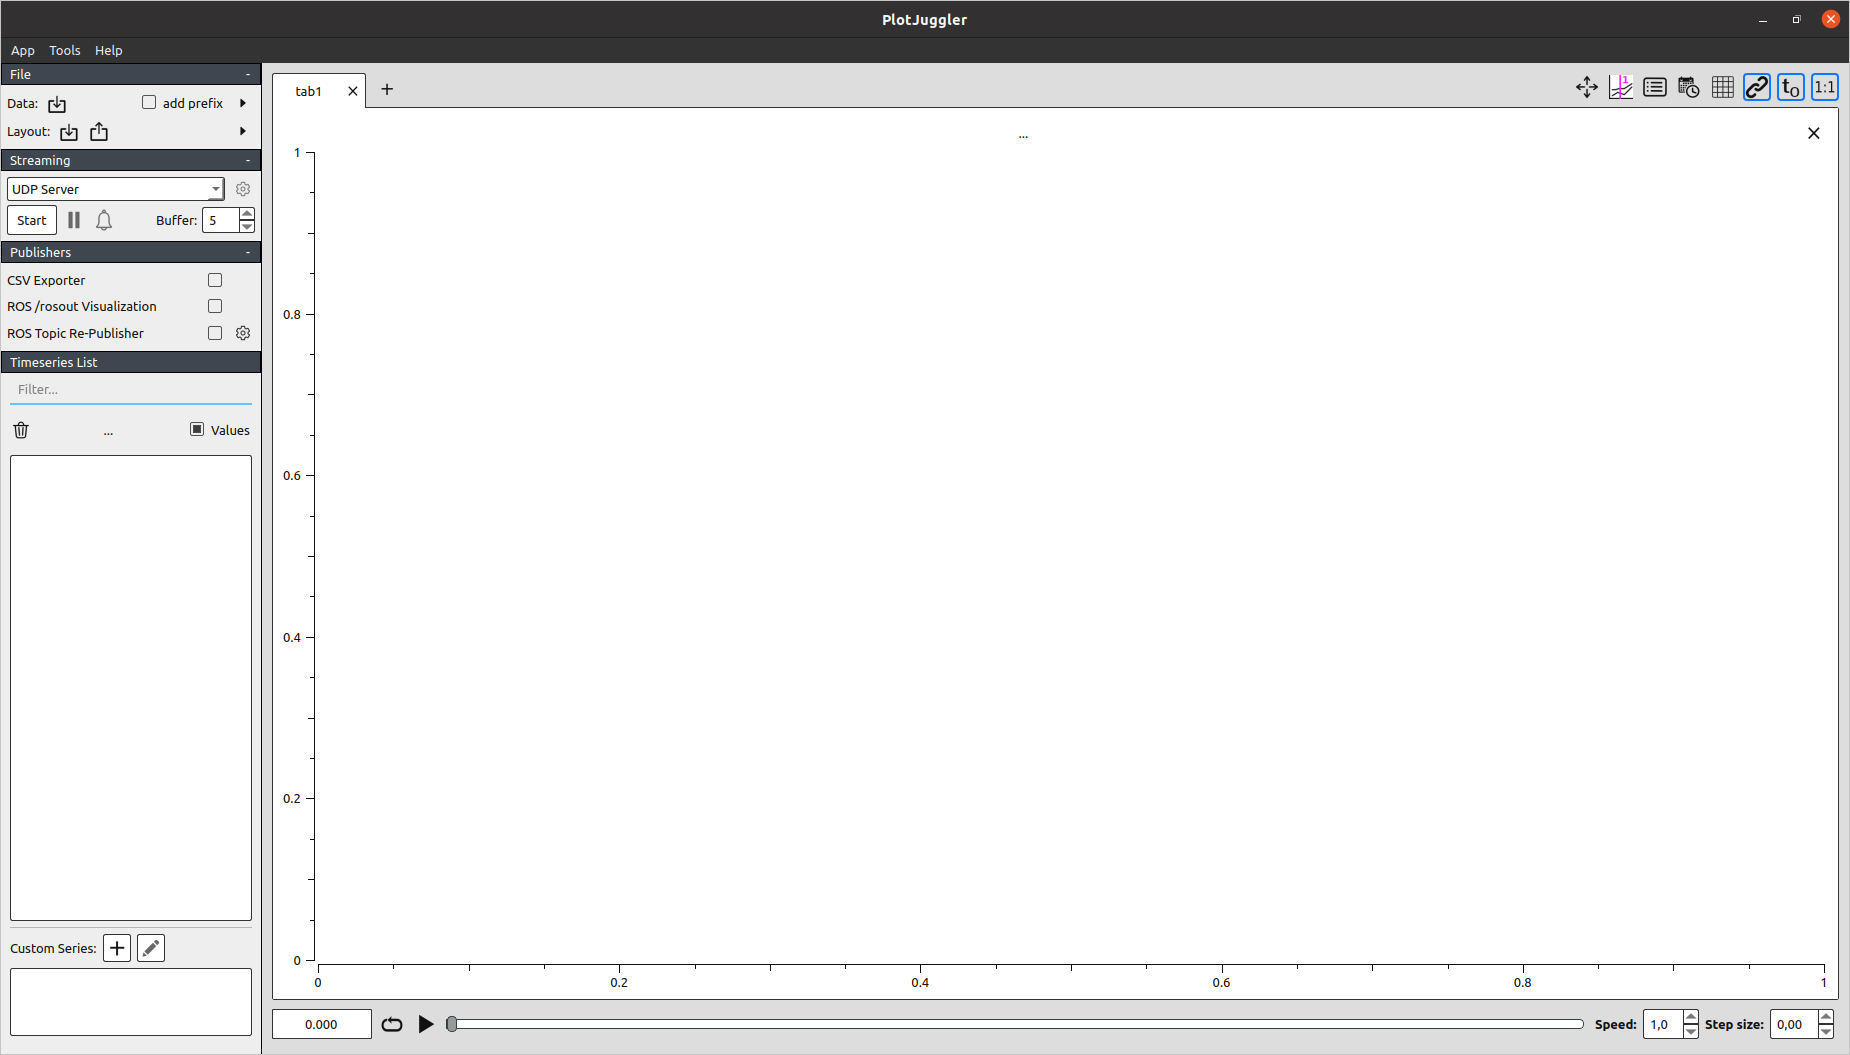
\includegraphics[width=\textwidth]{plotjuggler.png}
    \caption{Plotjuggler}
    \label{fig:plotjuggler}
\end{figure}

In the dropdown menu under \textit{Streaming}, pick \textbf{ROS topic subscriber}. Make sure you are connected to the RPi via ethernet, and click start. If you are prompted for the location of the ROS\_MASTER, set it to: \textit{http://192.168.1.2:11311}. You may have to do this in the command window before you start Plotjuggler as well. Then the command is: 

\begin{lstlisting}[language=bash,basicstyle=\mlttfamily, breaklines=true]
  $ export ROS_MASTER_URI=http://192.168.1.2:11311
\end{lstlisting}

After pressing start you will get a list of available topics. Pick the relevant ones and pull them into the coordinate system to view the live feedback. 

\section{Dynamic Reconfigure}

To make tuning your controller and observer more effective, tools for dynamic tuning are provided in the form of the ROS-package gain\_server. This allows you to change the gains in real time, rather than having to hard-code the gains and then stopping and starting your simulation every time you want to change them. To activate the node, and GUI use the following steps: 

\begin{itemize}
    \item Make sure you have imported the Gains object from lib.py. It is built like most other objects and contais get-methods for extracting gains, along with callback-functions.
    \item In the \textbf{observerInitNode()} or \textbf{controllerInitNode} uncomment the line starting with \textit{gain\_client}.
    \item To run the node use the command:
    \begin{lstlisting}[language=bash,basicstyle=\mlttfamily, breaklines=true]
    $ rosrun gain_server server.py
    \end{lstlisting}
    \textbf{NOTE!} If you use the dynamic tuning, you should always activate this node \textbf{first} or you may experience errors. This is because the observer and controller nodes will expect values to be there when they are not. When the node is activated, the initial gains should be printed to your terminal
    \item In another terminal, activate the GUI: 
     \begin{lstlisting}[language=bash,basicstyle=\mlttfamily, breaklines=true]
    $ rosrun rqt_gui rqt_gui -s reconfigure
    \end{lstlisting}
    
    This should open a program that looks like this: 
    
    \begin{figure}[h]
        \centering
        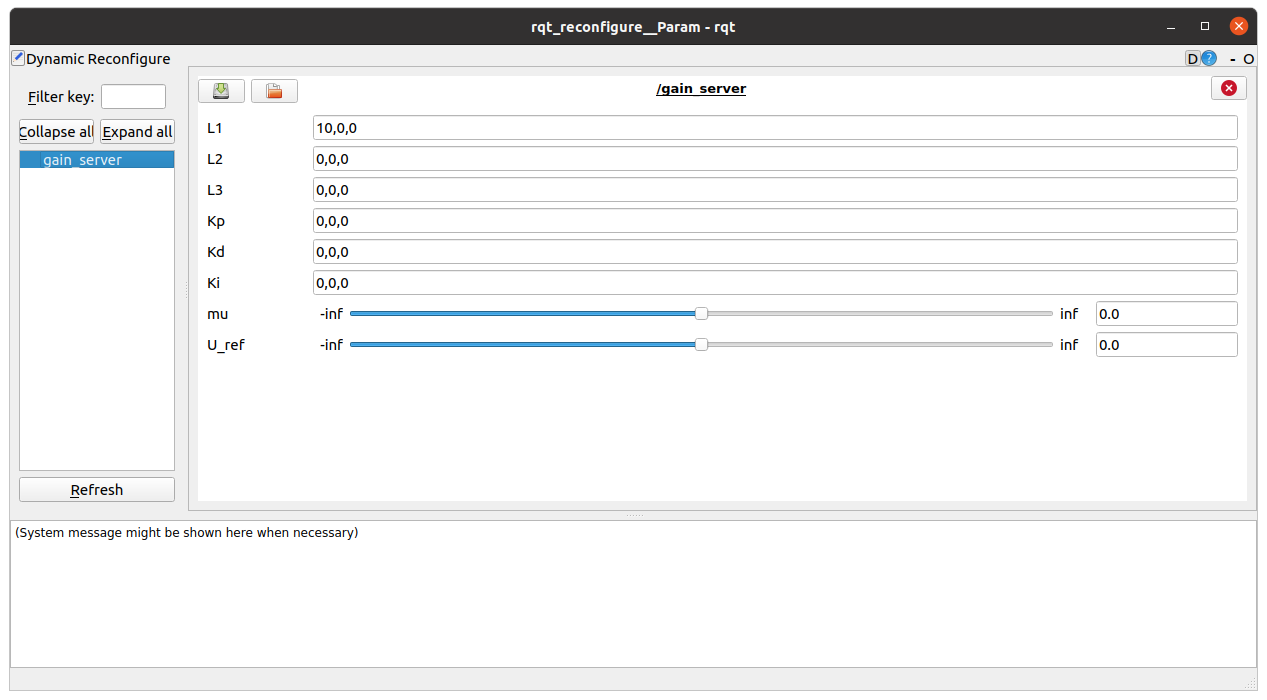
\includegraphics[width=\textwidth]{dynamic-reconfigure.png}
        \caption{Tuning GUI}
        \label{fig:tuner}
    \end{figure}
    
    Each field or slider here corresponds to a gain in either the observer or controller. Not all the variables are relevant either. The last to are single float values, while the first six are meant to represent the elements on the diagonal of a $3\times3$-matrix. Change these to tune you controller. 
\end{itemize}
\end{document}
